\documentclass[notes,intlimits]{beamer}

\mode<presentation>
{
  \usetheme[footline]{PISMshade}
  \setbeamercovered{transparent}
}

% load packages
\usepackage{multimedia}
\usepackage[english]{babel}
\usepackage[latin1]{inputenc}
\usepackage[T1]{fontenc}
\usepackage{lmodern}
\usepackage{pdfpages}
\usepackage[multidot]{grffile}

\usepackage{tikz}
\usetikzlibrary{shapes,arrows}
\usetikzlibrary{shadows}
\usetikzlibrary{mindmap}

\definecolor{dark red}{HTML}{E41A1C}
\definecolor{dark green}{HTML}{4DAF4A}
\definecolor{dark violet}{HTML}{984EA3}
\definecolor{dark blue}{HTML}{084594}
\definecolor{dark orange}{HTML}{FF7F00}
\definecolor{light blue}{HTML}{377EB8}
\definecolor{light red}{HTML}{FB9A99}
\definecolor{light violet}{HTML}{CAB2D6}

\setbeamercolor{boxed}{fg=black,bg=light blue!25}
\graphicspath{{figures/}}

\setbeamertemplate{background canvas}
{
  \tikz{\node[inner sep=0pt,opacity=1.0]
    {
\includegraphics[width=\paperwidth]{pism_beamer_shade_bg}};}
}

% title page
\title{PISM: What does it do? And how does it work?}

\author{C.~Khroulev}

\date{}

\subject{The Parallel Ice Sheet Model}

\begin{document}

% insert titlepage
\begin{frame}
  \titlepage
\end{frame}

\setbeamertemplate{background canvas}{} 

\section{Overview}
\label{sec:overview}

\begin{frame}{The basics}
  \begin{itemize}
  \item uses a uniform Cartesian grid
  \item High-resolution runs use a large number of unknowns, requiring
    parallel I/O.
  \item ... and a parallel domain decomposition to avoid running out
    of memory
  \end{itemize}
\end{frame}

\note{
  The fact that is uses a uniform grid means that it has to
  keep track of more unknowns compared to a model using an
  adaptive mesh, but its output is easier to analyze because it
  does not require post-processing.

  Compute the number of unknowns in a high-ish resolution
  Greenland simulation.

  A figure showing domain decomposition would be useful.

  This is where I would mention ``ghosts'' and that we ne
  ensure that they are up to date, if I thought that it needs
  mentioning.
}

\begin{frame}{Free boundaries}
  Both ice thickness and its extent can change, meaning that PISM has
  to deal with two kinds of free boundaries:

  \begin{itemize}
  \item lateral (in the map plane)
  \item at the top surface
  \end{itemize}
\end{frame}

\note{
  Lateral: a cell is either icy or not, except for ``partially-filled'' cells.
}

\begin{frame}{Free boundary at the top surface and the vertical coordinate}
  There are two common approaches:
  \begin{itemize}
  \item sigma-coordinate (used by some other models, e.g. SICOPOLIS)
  \item ``immersed'' top boundary plus a transformed
    vertical coordinate (used by PISM)
  \end{itemize}
\end{frame}

\note{
  Sigma-coordinate: top boundary follows ice geometry as it
  evolves. Requires modifying most equations (except for shallow,
  two-dimensional ones).

  The surface $z=0$ follows the base of the ice. In general,
  $z=C$ is not a plane; see the Manual for the corresponding
  changes in energy balance equations.
}

\section{Sub-models}
\label{sec:sub-models}

\begin{frame}{Sub-models}

  % PuBu
  \definecolor{levelo}{RGB}{5,112,176}
  \definecolor{leveli}{RGB}{116,169,207}
  \definecolor{levelii}{RGB}{189,201,225}
  \definecolor{leveliii}{RGB}{241,238,246}

  \begin{center}
    \scalebox{0.55}{
      \begin{tikzpicture}[mindmap, concept color=levelo, font=\sf, text=black]

        \tikzstyle{level 1 concept}+=[font=\sf, sibling angle=40]

        \node[concept] {PISM}
        [clockwise from=0]
        child[concept color=leveli]{
          node[concept]{Geometry evolution}
          [clockwise from=60]
          child[concept color=levelii]{ node[concept]{Mass transport} }
          child[concept color=levelii]{ node[concept]{Calving} }
          child[concept color=levelii]{ node[concept]{Iceberg elimination} }
        }
        child[concept color=leveli]{
          node[concept]{Energy balance}
          [clockwise from=-60]
          child[concept color=levelii]{ node[concept]{Bedrock thermal layer}}
        } 
        child[concept color=leveli]{ node[concept]{Stress balance} } 
        child[concept color=leveli]{ node[concept]{Bed deformation} } 
        child[concept color=leveli]{ node[concept]{Age} }
        child[concept color=leveli]{ node[concept]{Subglacial hydrology} }
        child[concept color=leveli]{ node[concept]{Sea level forcing} }
        child[concept color=leveli]{ node[concept]{Sub-shelf boundary conditions} }
        child[concept color=leveli]{
          node[concept]{Top surface boundary conditions}
          [clockwise from=60]
          child[concept color=levelii]{ node[concept]{Atmosphere model} }
        }
        ;
      \end{tikzpicture}
    }                           %scalebox
  \end{center}
\end{frame}

\note{
  These are the parts PISM consists of, conceptually.
}

\begin{frame}{Universal considerations}
  \begin{itemize}
  \item inputs and outputs
  \item initialization
  \item ``bootstrapping'' (initialization from incomplete input data)
  \item time stepping restrictions
  \item computational costs
  \item modeling challenges
  \end{itemize}
\end{frame}

\section{Time stepping}
\label{sec:time-stepping}

\begin{frame}{Explicit time stepping}

\begin{enumerate}
  \item use stress balance to compute velocity
      \begin{itemize}
      \item often: first get $(u,v)$, then $w$ from incompressibility
      \end{itemize}
  \item somewhere in here do other processes: thermodynamics, basal melt, calving, \dots
  \item decide on time-step $\Delta t$ from diffusivity $D$ \hfill (\emph{or: fixed} $\Delta t$)
  \item from velocity, surface balance, and base balance do time-step of mass continuity equation to get $H_t$
  \item update surface elevation: $h \gets h+H_t \Delta t$
  \item repeat at 1.
\end{enumerate}

\bigskip
\begin{itemize}
\item this paradigm \emph{is} explicit time stepping of the whole model
\end{itemize}
\end{frame}

\section{Geometry evolution}
\label{sec:geometry-evolution}

\begin{frame}{Mass transport}
  \begin{itemize}
  \item uses the finite-volume approach
  \item tailored to take advantage to PISM's split between
    ``diffusive'' and ``advective'' ice flow
  \item ice flow is diffusive, so numerical diffusivity does not cause
    much trouble
  \item surface and basal mass balance may be negative and extra care
    is needed to preserve non-negativity of ice thickness
  \end{itemize}
\end{frame}

\note{ Alternative: coupled stress balance and mass continuity with an
  inequality constraint, i.e. the variational inequality formulation.
}

\begin{frame}{Stability considerations}
  The SIA flow is diffusive, so preserving staility of explicit time
  stepping forces us to respect diffusion-related time step
  restrictions.

  FIXME: use equations to show that SIA \textbf{has} a diffusion.

  This applies to other models, even if they don't use the shallow ice
  approximation.

  This stability requirement forces PISM to take short time steps.
\end{frame}

\begin{frame}{Free boundary at the calving front}
  Using parially-filled cells to model moving calving fronts.

  FIXME: add a figure from Torsten's paper.
\end{frame}

\begin{frame}{Calving}
  \begin{itemize}
  \item Geometric criteria
    \begin{itemize}
    \item ice thickness threshold
    \item floating ice
    \item prescribed maximum shelf extent
    \end{itemize}
  \item Stress-based
    \begin{itemize}
    \item Eigencalving (FIXME: formula and reference)
    \item von Mises (FIXME: formula and reference)
    \end{itemize}
    Challenges: strain rates estimated using finite differences may be
    of poor quality
  \end{itemize}
\end{frame}

\begin{frame}{Iceberg elimination}
  Why do we need this?

  \begin{itemize}
  \item The SSA stress balance determines the sliding velocity of
    patches of floating ice \emph{up to rigid body motions} (see C.
    Schoof, \emph{A variational approach to ice stream flow})
  \item We need to keep track of an ice sheet's discharge into the
    ocean.
  \end{itemize}

  Where would an ``iceberg'' (isolated patch of floating ice) come
  from?
  \begin{itemize}
  \item calving
  \item sea level changes
  \end{itemize}
\end{frame}

\begin{frame}{Iceberg elimination: technical details}

  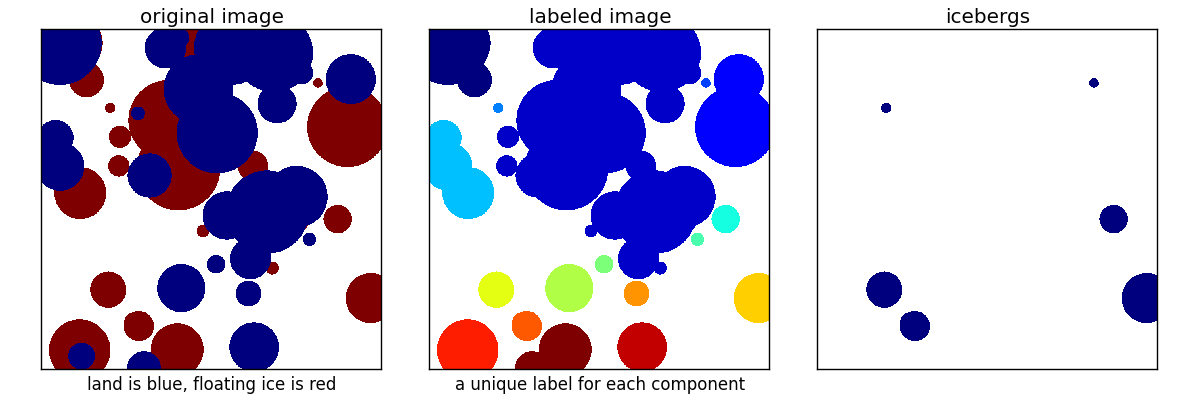
\includegraphics{icebergs.png}

  \begin{itemize}
  \item 
  \end{itemize}
\end{frame}

\end{document}